\section{Physical layer in \mbox{Mote Runner}}
\begin{frame}[fragile]
  \frametitle{Radio interface}
  \begin{itemize}
    \item MR v.13 offers a Radio interface IEEE 802.15.4 compliant
    \begin{itemize}
    	\item It is a generic class in the IBM saguaro system that permits to use the radio device
    	\item It offers an API with the following functionality:
    	\begin{itemize}
			\item open: opens the radio, once opened no other assembly can use it
			\item close: releases the radio so that others can use it
			\item setter and getters for channel and network parameters (addresses, panid...)
			\item startReceive: listens the channel (in one of the many receiption mode)
			\item transmit: begin to transmit a pdu
    	\end{itemize}
    \end{itemize}
  \end{itemize}
\end{frame}

\begin{frame}[fragile]
	\frametitle{Radio interface}
	\begin{itemize}
		\item In addition Radio:
		\begin{itemize}
			\item Handles transmission and reception notifying to higher level by delegation, registering functions that will handle the events (tx and rx)
			\item Manages acks notifying states of failure or success to callbacks
			\item Permits to set parameters as PAN identifier, short address, radio channel
		\end{itemize}
	\end{itemize}
\end{frame}


\begin{frame}[fragile]
  \frametitle{Transmission \& Reception}
  \begin{itemize}
    \item These operations require much attention:
    \begin{itemize}
    	\item Radio permits to transmit every type of pdu, but it's possible to receive only packets with 802.15.4 well formed headers
    	\item Receiving in promiscuous mode allows to receive every kind of packet, but this exposes to interferences
    \end{itemize}
    \item Each mote holds 3 addresses:
    \begin{itemize}
    	\item a 16-bit PAN identifier
    	\item a 64-bit extended address that uniquely identifies a mote (EUI-64)
    	\item a 16-bit short address that's application and protocol specific
    \end{itemize}
  \end{itemize}
\end{frame}

\begin{frame}[fragile]
  \frametitle{Transmission \& Reception}
  \begin{figure}
  	\centering
  	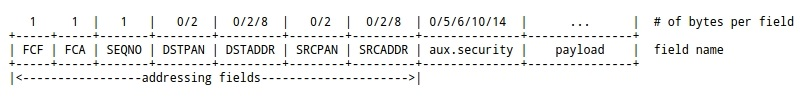
\includegraphics[width=\textwidth]{img/header.jpg}
  	\caption{PDU header format}
  \end{figure}
  \begin{columns}
  	\begin{column}{.52\textwidth}
	    \begin{figure}
	    	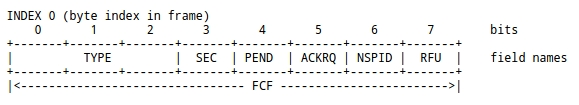
\includegraphics[width=\textwidth]{img/fcf.jpg}
  		\caption{Frame Control Flags}
	    \end{figure}
  	\end{column}
  	\hfill
	\begin{column}{.45\textwidth}
	    \begin{figure}
	    	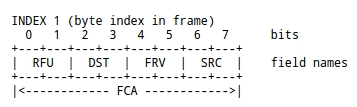
\includegraphics[width=\textwidth]{img/fca.jpg}
  		\caption{Frame Control Address Flags}
	    \end{figure}
  	\end{column}
  \end{columns}
\end{frame}
% 
% \begin{frame}[fragile]
%   \frametitle{Tx/Rx - Filtering}
%   \begin{itemize}
%     \item Possible packets are specified in FCF-Type field and are: BEACON, DATA, ACK and CMD.
%     \item BEACONs are accepted only if the header field SRCPAN matches the mote's PANID or it's BROADCAST
%     \item If FCA Flags specify an address then 
%   \end{itemize}
% \end{frame}

\begin{frame}[fragile]
  \frametitle{Tx/Rx and Real Time Constraints}
  \begin{itemize}
    \item It's possible to operate in many different ways with regards to real time constraints:
    \begin{itemize}
    	\item ASAP, EXACT, TIMED, RX4EVER indicate when the operation should begin and/or end given two time instant
    	\item MR manages autonomously all warm up and ramp up to make the device ready given one of these modes
    	\item At the end the device turns off and an event is raised to be managed with delegation
    	\item If the device cannot be ready or cannot complete a task within the specified time an error occurs
    \end{itemize}
  \end{itemize}
\end{frame}